\chapter{Accretion Disc Winds}
\label{sec:winds}

\epigraph{``A view of space, with an elephant obstructing it"}
{{\sl Mike Vennart, Silent/Transparent}}


%%%%WINDS 
%%% COULD MAKE THIS A NEW CHAPTER
\section{Observational Evidence}

Observational evidence for mass-loaded outflows or winds is 
widespread across the entire astrophysical mass range and most of
the electromagnetic spectrum. Before exploring this evidence, 
it is pertinent to briefly discuss the `smoking gun'
used to unambiguously detect winds -- the presence of blue-shifted BALs
or `P-Cygni' profiles in an object's spectrum. 

\begin{figure}
\centering
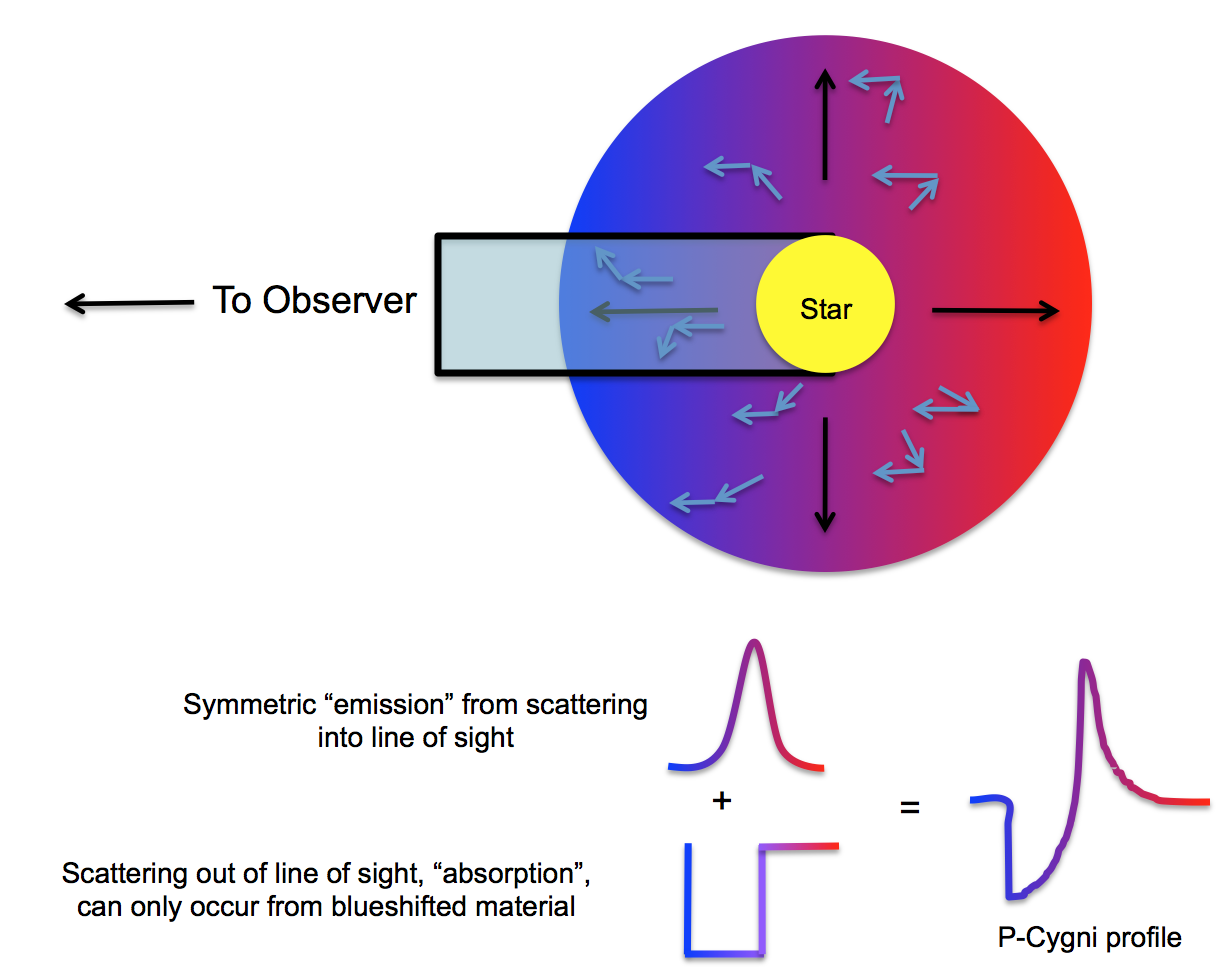
\includegraphics[width=1.0\textwidth]{figures/02-outflows/pcyg.png}
\caption
[A disagram showing how P-Cygni profiles form.]
{
Diagram showing how an expanding envelope or wind presenting significant line
opacity around a continuum source leads to the formation of P-Cygni profiles.
The black arrows denote the outflow direction and the blue arrows typical
scattering interactions.
} 
\label{fig:pcyg}
\end{figure}

Fig.~\ref{fig:pcyg} shows how a spherical outflow presenting
significant line opacity will 
cause these characteristic profile shapes to form, 
as scattering out of the line of sight 
causes a dip in the blue wing of the line, while scattering into the 
line of sight from other portions of the outflow causes an increase in flux
in the red wing of the line. The situation is much more complex in most
astrophysical situations; for example, the geometry is rarely spherically 
symmetric, and the line is rarely a pure scattering case. 
Indeed, the potential 
for complicated radiative transfer effects and 
the variety in line formation mechanisms 
(e.g. recombination, collisionally excitation)
is one of the reasons why 3D Monte Carlo radiative 
transfer simulations are necessary
to effectively model disc winds (see chapter 3).



\subsection{Cataclysmic Variables}

It has been known for a long time that winds emanating from
accretion discs are important in shaping the ultraviolet (UV) spectra
of high-state CVs \citep{heap1978, greensteinoke1982}. 
The most spectacular evidence for such
outflows are the P-Cygni-like profiles seen in UV resonance lines such as
\civfull\ \citep[e.g. ][see Fig.~\ref{fig:cordova}]{cordova1982}. 
Considerable effort has been spent over the
years on understanding and modelling these UV features 
\citep[e.g.][]{drewverbunt1985,maucheraymond1987,SV93,KWD95,
kd1997,knigge1997,LK02,noebauer,puebla2011}. 
The basic picture emerging from these efforts is
of a slowly accelerating, moderately collimated bipolar
outflow that carries away $\simeq 1\% - 10\%$ of the accreting
material. State-of-the-art simulations of line formation in this type
of disc wind can produce UV line profiles that are remarkably similar
to observations, as shown in Fig.~\ref{fig:zcam_lk02}.

\begin{figure}
\centering
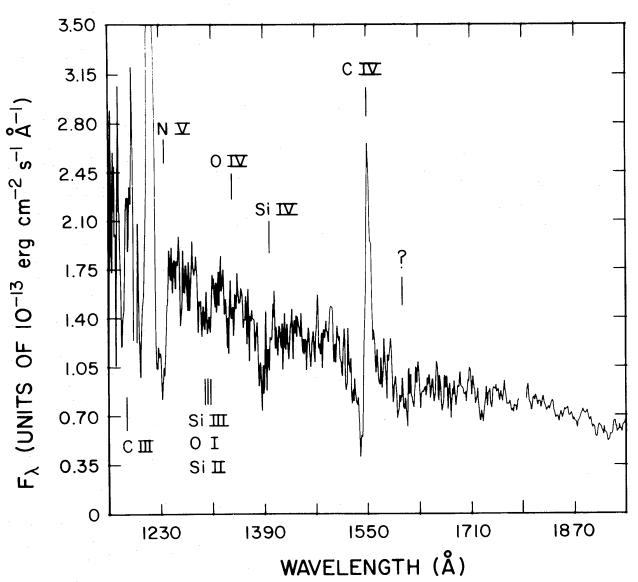
\includegraphics[width=0.8\textwidth]{figures/02-outflows/cordova_mason.png}
\caption
[UV spectrum of the DN TW Vir during outburst.]
{
{\sl Credit: Cordova \& Mason 1982}. 
UV spectrum of the DN TW Vir during outburst. The P-Cygni profiles
can be seen clearly, demonstrating that a strong, fast outflow is present
in the system. 
} 
\label{fig:cordova}
\end{figure}

\begin{figure}
\centering
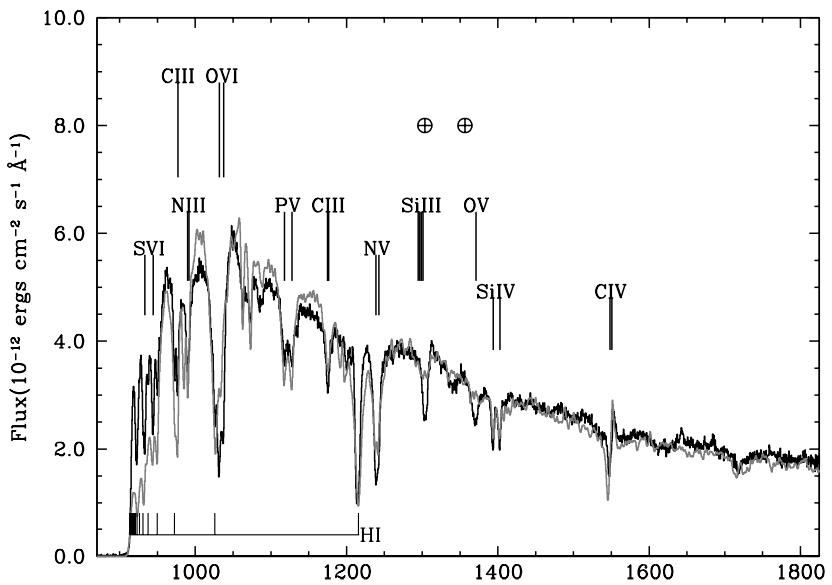
\includegraphics[width=0.8\textwidth]{figures/02-outflows/zcam_lk02.png}
\caption
[UV spectrum of Z Cam, compared to a synthetic spectrum from MCRT simulations.]
{
{\sl Credit: Long \& Knigge 2002}. 
UV spectrum of Z Cam, compared to a synthetic spectrum from MCRT simulations.
} 
\label{fig:zcam_lk02}
\end{figure}

\begin{figure}
\centering
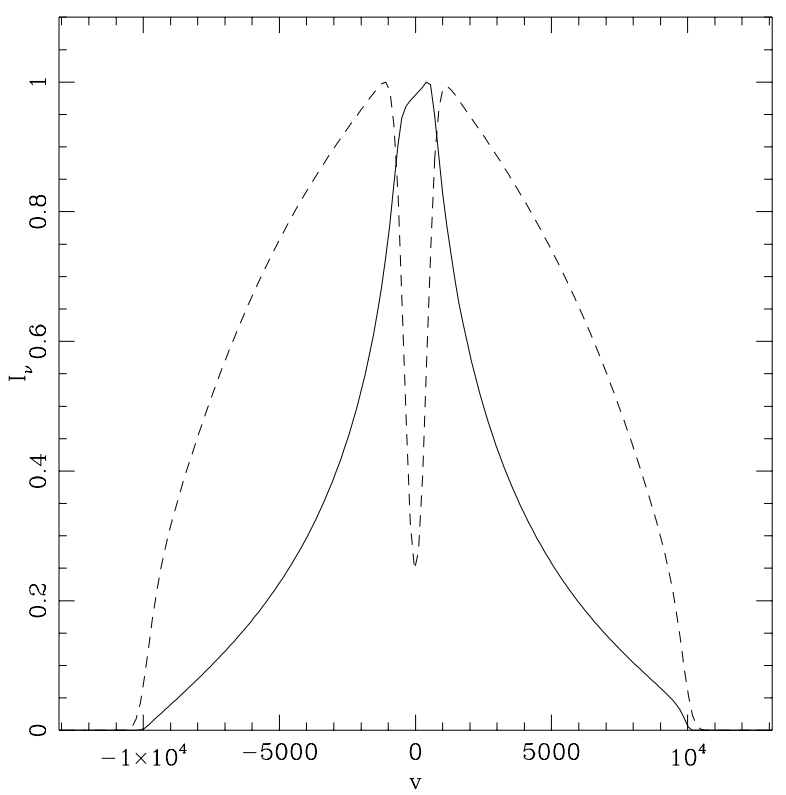
\includegraphics[width=0.7\textwidth]{figures/02-outflows/mc_line.png}
\caption
[The effect of a disc wind on a double-peaked line profile.]
{
{\sl Credit: Murray \& Chiang (1997)}. 
A comparison between a line profile, normalised to have peak intensity of 1,
produced from a Keplerian disk (solid line) and the same model with an additional
disc wind (dashed line). The radial velocity component of the disc wind modifies
the escape probabilities across the disc, causing a single-peaked line to form.
} 
\label{fig:mc_line}
\end{figure}

Much less is known about the effect of these outflows on the optical
spectra of high-state CVs. Direct evidence of wind-formed lines comes from
isolated observations of P-Cygni-like line profiles in
\ha\ and He \textsc{i} $\lambda5876$, 
\citep{patterson1996, RN98, kafka2004}. 
However, the effect of a wind  on the {\em emission} lines in the optical 
spectrum is unclear.
\cite{MC96, MC97} have shown that the presence of disc winds may
offer a natural explanation for the single-peaked optical emission lines in
high-state CVs, since they can strongly affect the radiative transfer
of line photons \citep[Fig.~\ref{fig:mc_line}; also see][]{flohic2012}. 
Stronger support for a significant wind contribution to the
optical emission lines comes from observations of eclipsing
systems. There, the single-peaked lines are often only weakly
eclipsed, and a significant fraction of the line flux remains visible
even near mid-eclipse \citep[e.g.][]{baptista2000,groot2004}. 
This points to line formation in a spatially
extended region, such as a disc wind.
It is also possible that a wind may affect the continuum emission of CVs,
as described in section~\ref{sec:disc_continuum}. 
The effect of an accretion disc wind
on the optical line and continuum emission of CVs is addressed directly
in chapter 4.

% These spectra are typically characterized
% by H and He emission lines superposed on a blue continuum. In many
% cases, and particularly in the SW~Sex subclass of NLs
% \citep{HSK86,DR95}, these lines are single-peaked. This is contrary to
% theoretical expectations for lines formed in accretion discs, which
% are predicted to be double-peaked \citep{smak1981, hornemarsh1986}. 
% {\em Low-state} CVs (dwarf novae in quiescence) do, in fact,
% exhibit such double-peaked lines \citep{marshhorne1990}. 

% Could disc winds also have an impact on the UV/optical {\em continuum}
% of high-state CVs? This continuum is usually thought to be dominated
% by the accretion disc and modelled by splitting the disc into
% a set of concentric, optically thick, non-interacting annuli following
% the standard $T_{eff}(R) \propto R^{-3/4}$ radial temperature
% distribution \citep{shakurasunyaev1973}. In such
% models, each annulus is taken to emit either as a blackbody or,
% perhaps more realistically, as a stellar/disc atmosphere model
% \citep{Schwarzenberg-Czerny1977,wade1984,wade1988}.
% In the latter case, the local surface gravity, $\log{g}(R)$, is
% assumed to be set solely by the accreting WD, since self-gravity is
% negligible in CV discs.

\subsection{X-ray Binaries}
\label{sec:xrb_winds}

As in CVs, evidence for fast outflows in LMXBs is not constrained to 
a single waveband. UV absorption in outflows was detected when
\cite{ioannau2003} observed \civfull\ P-Cygni profiles with blueshifts 
of $\sim1500$km~s$^{-1}$ in the LMXB X2127+119. 
A series of studies also found X-ray absorption features in similar objects 
\citep{ueda1998,kotani2000,parmar2002}. 
These absorption features appeared to be preferentially detected
in high-inclination, `dipping' LMXBs. This was confirmed
by \cite{ponti2012}, who proposed an equatorial outflow 
geometry based on this association (see Fig.~\ref{fig:ponti_cartoon}). 
The same study demonstrated that
the winds only appeared in the soft, 
disc dominated accretion state, on the opposite side of the HID to the
region where jets are common (Fig.~\ref{fig:ponti_hid}). 
This exciting result illustrates how
important winds are to our understanding of accretion, and requires that
we expand the discussion of accretion states from `disc-jet' coupling
to also include winds.

\begin{figure}
\centering
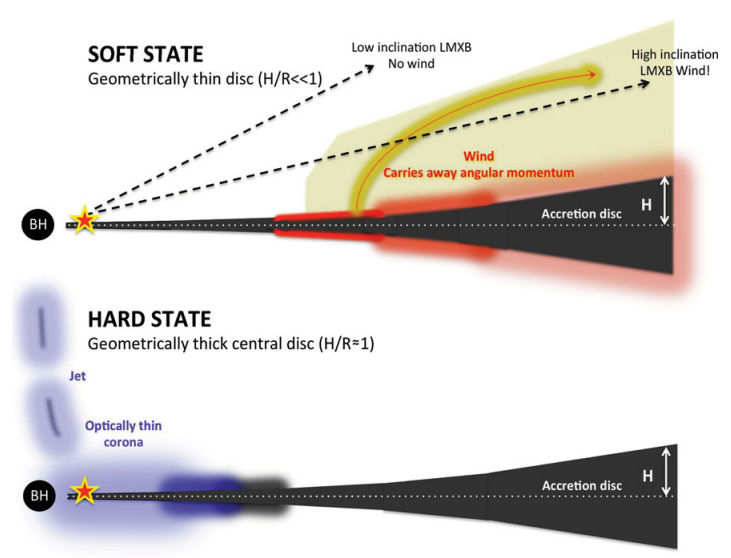
\includegraphics[width=0.8\textwidth]{figures/01-intro/ponti_wind_cartoon.png}
\caption
[A cartoon illustrating the expected geometry of soft-state LMXB winds.]
{
{\sl Credit: Ponti et al. 2012}. 
A cartoon illustrating the expected geometry of soft-state LMXB winds.
} 
\label{fig:ponti_cartoon}
\end{figure}


\begin{figure}
\centering
\includegraphics[width=0.8\textwidth]{figures/01-intro/ponti_hid.png}
\caption
[Hardness-intensity diagram for four dipping LMXBs.]
{
{\sl Credit: Ponti et al. 2012}. 
Hardness-intensity diagram for four dipping LMXBs,
demonstrating that winds appear only in the soft state.
} 
\label{fig:ponti_hid}
\end{figure}


\subsection{AGN and Quasars}
\label{sec:agn_winds}

\subsubsection{Broad Absorption Line Quasars}

\begin{figure}
\centering
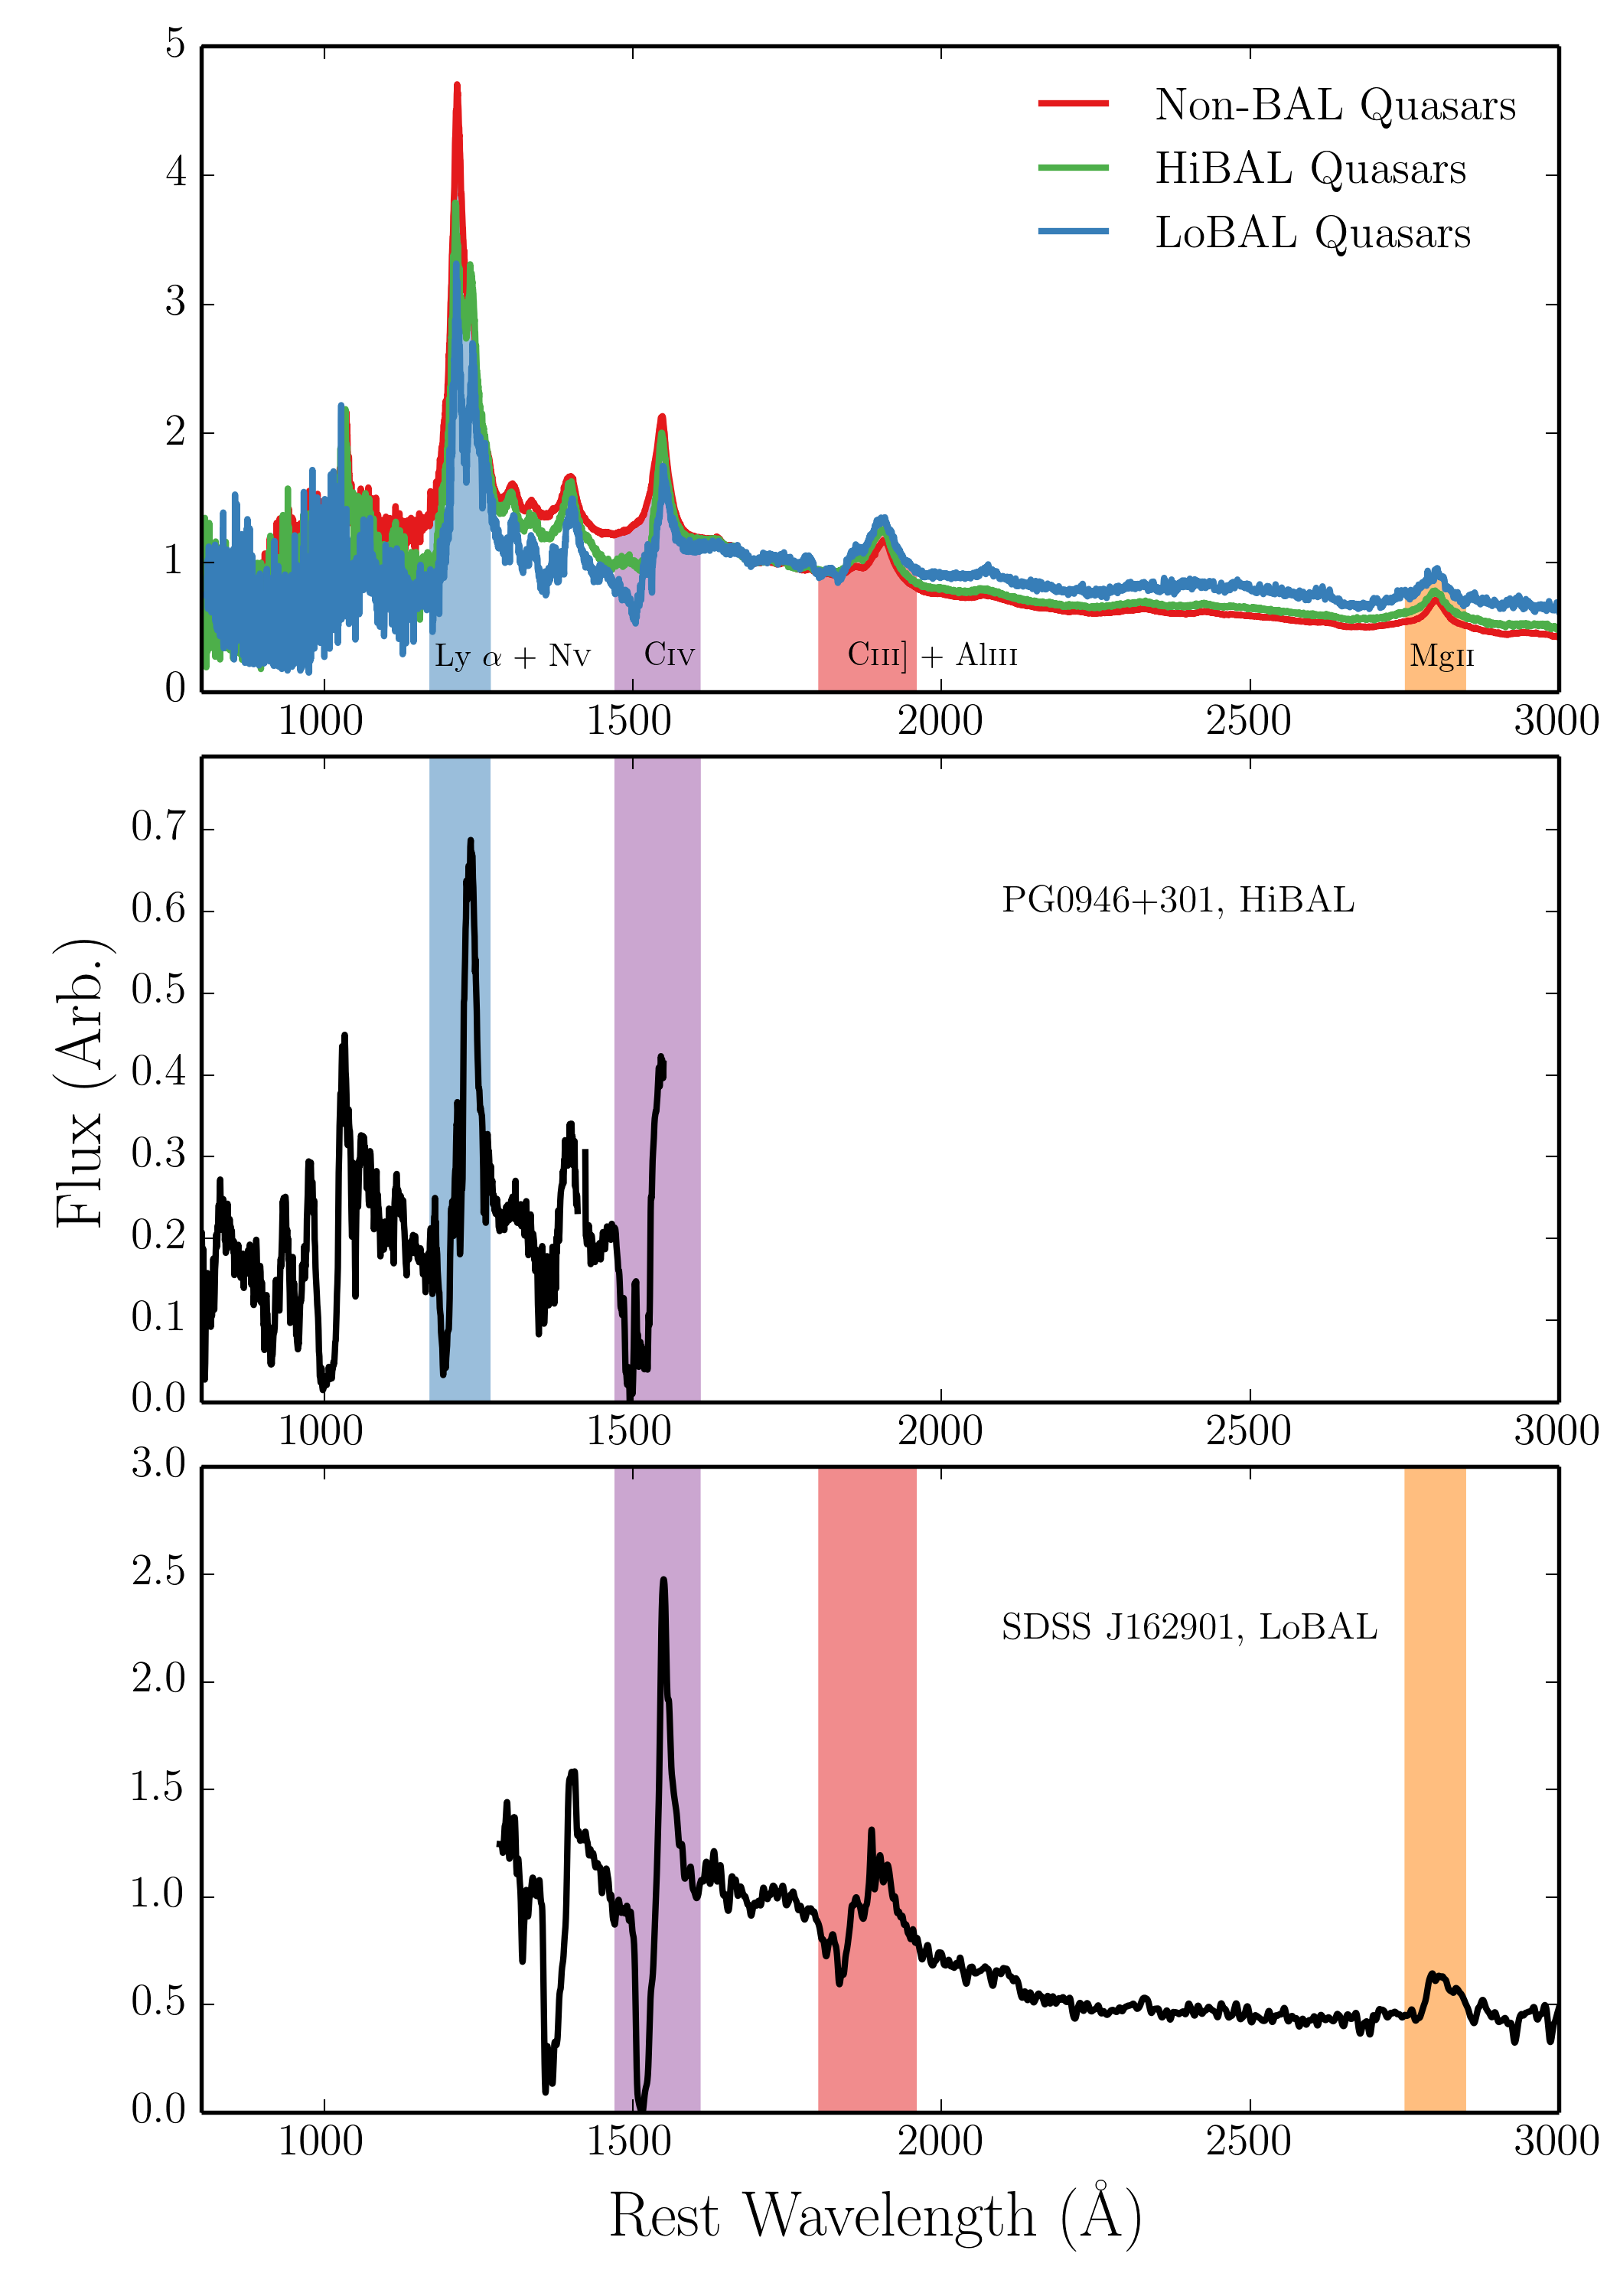
\includegraphics[width=1.0\textwidth]{figures/02-outflows/bal_spectra.png}
\caption
{
Five examples of BAL quasar spectra, from HST and SDSS.
} 
\label{fig:bals}
\end{figure}

Perhaps the clearest evidence of outflows in AGN is provided by  
the blueshifted ($\sim 0.1~c$) ultraviolet 
BALs seen in approximately $20\%$ of quasars
\citep{weymann1991, knigge2008, dai2008, allen2011}. Five example
spectra of BAL quasars from the HST and SDSS archives are shown in 
Fig.~\ref{fig:bals}. In addition to the more common high-ionization
BAL quasars (HiBALs), approximately $10\%$ of BALQSOs show absorption
in lower ionization species such as \mgii\ and \aliii\ 
\citep[LoBALs;][]{voit1993,gibson2009}
and an even smaller subset also show absorption in Fe~\textsc{ii} and 
\textsc{iii} \citep[FeLoBALs;][]{becker2000,hall2002}. 

The simplest explanation for the incidence of 
BAL quasars (BALQSOs) is in terms of an accretion disc wind viewed
from different angles. This principle of geometric unification
is very similar to the idea behind the UP95 and AM95 models discussed in Chapter 1.
According to this paradigm, a biconical wind rises from 
the accretion disc so that the BALQSO fraction is associated with
the covering factor of the outflow. This fraction
has been estimated by various authors using different 
selection criteria, with
values ranging between $10\%$ and $40\%$ depending on the treatment 
of selection effects and the classification scheme used 
\citep{weymann1991, trump2006, knigge2008, dai2008, allen2011}

BAL quasars can also be interpreted in an {\em evolutionary}
context, in which quasars spend a certain proportion of their life
in the `BAL phase'. Models generally put this phase near the start
of the quasar lifetime 
\citep{hazard1984,surdej1987,boroson1992,zubovas2013}, 
after a dust-enshrouded phase, but before
the main quasar period. It is perhaps more likely that {\em both} 
evolutionary and geometric effects are at work \citep{borguet2010,dai2012}.
One of the main problems with testing these two paradigms is that many of
the properties of BAL quasars fit naturally into either picture, and so
disentangling their true nature is challenging. 
The latter chapters of this thesis attempt to address this issue by testing the 
geometric unification model
and seeing how close this simple picture can get to explaining 
the BAL phenomenon.  

While the BAL fraction, $f_{BAL}$, is a very useful number and must be at least
related to the covering factor of the outflow, continuum selection
effects \citep{goodrich1997,krolikvoit1998}, 
as well as reddening \citep{allen2011}, could significantly
bias $f_{BAL}$ estimates. The degree of collimation of the BAL wind
is also not well known. Polarisation studies suggest that the 
wind is roughly equatorial \citep{goodrich1995, cohen1995}, 
as also found from hydrodynamical and radiative transfer simulations 
\citep{PSK2000,PK04, higginbottom2013},
but there is also evidence for polar BAL outflows in 
radio-loud (RL) sources \citep{zhou2006,ghoshpunsly2007}.
In addition to these uncertainties, the physical scale of the BAL
phenomenon is also disputed and may vary from object to object.
A common assumption is that the BAL region is roughly co-spatial with
the BLR, which is reasonable considering the similar velocity widths
and ionization states in BELs and BALs. In this case, 
the radius of the absorbing material
can be estimated as $\sim 100 r_G -1000 r_G$ from reverberation mapping
and microlensing \citep[e.g., for BLRs in BALQSOs,][]{sluse2015,odowd2015}.
However, distances of  $\sim0.1$~pc ($\sim 10^4 r_G$) 
have been estimated in at least some objects from photionization modelling, 
conducted using densities calculated from absorption line doublets
\citep{borguet2013,chamberlain2015}.

BAL quasars display a wide variety of different trough shapes, 
as shown in Fig.~\ref{fig:bals}. The 
line profiles themselves often show complex structure 
\citep{foltz1987,ganguly2006, simonhamann2010} and can be time variable 
\citep{hall2011, capellupo2011,capellupo2012,capellupo2014, filizak2012}. 
Furthermore, there are a set of quasar absorption systems that show
BAL-like absorption troughs with much smaller velocity widths. Depending 
on their width, these are known as narrow absorption lines (NALs) or `mini-BALs'
\citep{misawa2007,misawa2008,nestor2008}.
While some of this behaviour can be explained once again as a viewing angle
effect \citep[e.g. ][]{ganguly2001}, the range of 
BAL profile shapes suggests that they 
are far from a homogenous population, and may also possess
multi-scale substructures (clumps) in their flows. Clumping
is discussed in more detail in sections~\ref{sec:stellar_winds} and 
\ref{sec:rad_winds}, as well as in chapter 5.

The X-ray properties of BAL quasars are particularly important due
to the strong ionizing potential of the X-ray radiation. 
BALQSOs are X-ray weak when compared to 
non-BAL quasars \citep{gibson2009}. 
The X-ray weakness of BALQSOs is often attributed to X-ray absorption 
with column densities of $N_H \sim 10^{22-24}$~cm$^{-2}$ 
\citep{gallagher1999,gallagher2002,green2001,grupe2003,stalin2011},
although there is also evidence that BALQSOs are {\em intrinsically}
X-ray weak \citep{sabra2001,clavel2006,morabito2013}.
The X-ray properties of BAL quasars are fundamentally coupled to 
the properties of the wind -- the X-ray absorption may be caused by 
the outflow, which in turn has its ionization state 
determined by the X-ray radiation. Furthermore, the true X-ray 
luminosities cannot be reliably inferred until the 
inclinations of BALQSOs are
constrained, as gravitational lensing can significantly alter the
emergent angular distribution of X-ray emission even for an intrinsically
isotropic source \citep{chen2013a, chen2013b}.

Although the X-rays in BALQSOs are weaker than in similar mass quasars,
they still possess strong ionizing power. This leads to what has become
known as the `over-ionization problem' in BALQSOs: how is the moderate 
ionization state of the BAL gas maintained in the presence of ionizing 
X-rays? A number of potential solutions have been proposed, which can be 
broadly separated into `shielding' models \citep{MCGV95,PK04} and `clumpy'
models \citep{dekool1995,hamann2013}. Some of these models are discussed
further in section~\ref{sec:wind_models} and chapter~5.

\subsubsection{Warm Absorbers}

Warm absorbers (WAs) are regions of photoionized plasma responsible for some
of the characteristic absorption features seen in the 
X-ray spectra of AGN \citep{reynolds1995}.
In particular, they produce photoelectric continuum absorption 
\citep[e.g.][]{halpern1984,cappi1996,kriss1996}
and a series of narrow absorption lines in H-like and He-like ions of 
C, N, O, Si, Ne, and Fe \citep{kaastra2000}, that appear in the soft X-rays.
A wind origin is a common hypothesis for WAs 
\citep[e.g.][]{krolikkriss2001}. Clear evidence for this 
comes from the measured blueshifts of the lines, typically on the order of 
$\sim100$km~s$^{-1}$. X-ray absorption and WAs are often
variable \citep{fabian1994,otani1996}, which may be interpreted in terms of 
changing kinematics of an accretion disc wind \citep{connolly2014}. 
There is also evidence of contemporary UV and X-ray absorption 
in NGC 5548 \citep{kaastra2014} and mini-BALS \citep{giustini2011},
and as mentioned above BALQSOs 
are often absorbed in the X-rays. This suggests that the outflow phenomenon 
across a large range of ionization states and line energies is linked. 

Some WAs be modelled well with single component 
models \citep{kaastra2000}, but most
require multiple absorbers with different ionization states
\citep[e.g.][]{kriss1996,orr1997,krolikkriss2001,connolly2014}.
If this is the case, then self-consistent ionization and radiative transfer models
should really be used to model the spectrum (see e.g. chapter 3), 
as optically thin ionization parameter estimates will not capture 
the ionization and radiation physics.
The collated observations point towards some kind of outflow with a stratified ionization
structure, with $\log \xi \sim 0-2$, and densities on the order of $10^8$~cm. 
These physical conditions or scales are not well constrained, and the connection to 
other outflows is unknown. Timing observations may help to shed light on 
the properties of the mysterious, but ubiquitous, 
AGN WAs \citep{silva2015}.

\subsubsection{Ultra-fast Outflows}
\label{sec:ufos}

As well as acting as WAs, winds can also imprint clear absorption features
in highly ionized Fe~K$\alpha$ lines in AGN such as PDS~456 
\citep{reeves2003, gofford2014,matzeu2016},
MCG-5-23-16 \citep{braito2007} and PG 1211+143 \citep{poundsreeves2009,fukumura2015}.
These outflow signatures are fairly common in Seyfert galaxies \citep{tombesi2010a, gofford2013}. 
One example of such a feature is shown in 
Fig.~\ref{fig:nardini} along with a simple spherical outflow model fit 
\citep{nardini2015}. The high velocities ($\sim0.1c$) inferred 
from the line blueshifts have lead to these winds becoming known as 
ultra-fast outflows, or UFOs. 

UFOs are characterised by ionization parameters in the range $\log \xi \sim 3-4$
and column densities $N_H > 10^{22}$~cm$^{-2}$. Their high mass-loss rates
and large energy budgets mean that they are natural candidates for
AGN feedback (see section~\ref{sec:agn_feedback}). Measurements of
their kinetic luminosities suggest that UFOs have sufficient 
energy to affect their host galaxy \citep{gofford2015}. In fact, 
a large-scale molecular outflow has recently been detected in one 
UFO host, possibly driven by the UFO itself \citep{tombesi2015}. 
As with WAs, many of the models
used to constrain physical parameters are simplistic, and assume 
single ionization parameters, large covering factors
and thin expanding shells of outflow.
Under the assumption of a thin expanding shell, 
the mass-loss rate can be estimated using
\citep[e.g.][]{borguet2012}
\begin{equation}
\label{eq:hse}
\dot{M} \sim \Omega N_H m_p v_{out} R_{in},
\end{equation}
where $\Omega$ is the solid angle covered by the outflow, $N_H$
is the column density, $m_p$ is the proton mass, $v_{out}$ is the outflow velocity
and $R_{in}$ is the launch radius of the outflow.
In reality, the absorber is probably much more complex, and full 
RT and photoionization simulations are required to accurately model 
the expected spectrum. 
In a series of papers, 
\cite{simlong2008,sim2010_hydro,sim2010_hydro} carried out such calculations
and found that reasonable verisimilitude with Fe line profiles could be achieved.
However, as with many models of AGN, a holistic, broad wavelength range
fit is still required.

\begin{figure}
\centering
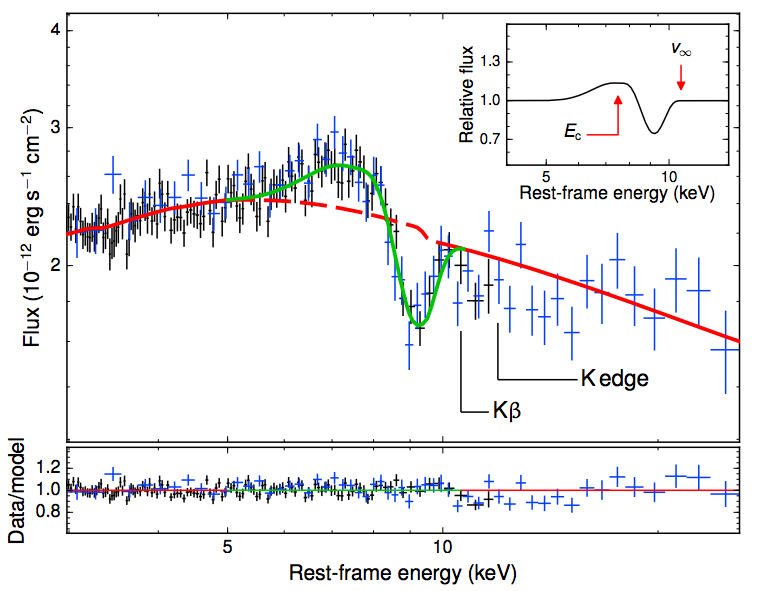
\includegraphics[width=1.0\textwidth]{figures/02-outflows/nardini_pds456.png}
\caption
[X-ray spectrum of PDS 456 fitted with a P-Cygni profile.]
{
{\sl Credit: Nardini et al. 2015}. 
X-ray spectrum of PDS 456 fitted with a P-Cygni profile from a 
spherical outflow model. {\sl XMM-Newton} data is shown in black 
with two combined {\sl NuStar} observations in blue.
} 
\label{fig:nardini}
\end{figure}


\subsection{Stellar Winds}

\label{sec:stellar_winds}

Although stellar winds are clearly not accretion disc winds,
they provide a useful, and better understood, testing ground for much
of the physics of radiatively-driven outflows. 
Wolf-Rayet (WR) stars and O-stars possess strong outflows with mass-loss rates
of up to $10^{-5}~M_\odot~$yr$^{-1}$, throught to be driven by radiation pressure
mediated by spectral lines (see section~\ref{sec:line_driving}). 
Over the typical lifetime of a massive
star ($\sim10^6$~yr), this can have a significant impact on the overall stellar mass,
causing losses of around $10~M_\odot$ of material. 

As with the systems described previously, the P-Cygni profiles
in spectra from hot, massive stars are the main pieces of evidence that
a strong wind is present (see Fig.~\ref{fig:hot_star_wind}). Mass-loaded
winds are also thought to be responsible for the emission lines 
seen in hot star spectra \citep[e.g.][]{pauldrach1994}. Indeed, emission
line diagnostics have been particularly important in determining
the mass-loss rates of stellar winds and have also been used to demonstrate 
that line-driven stellar winds are clumpy. 

\begin{figure}
\centering
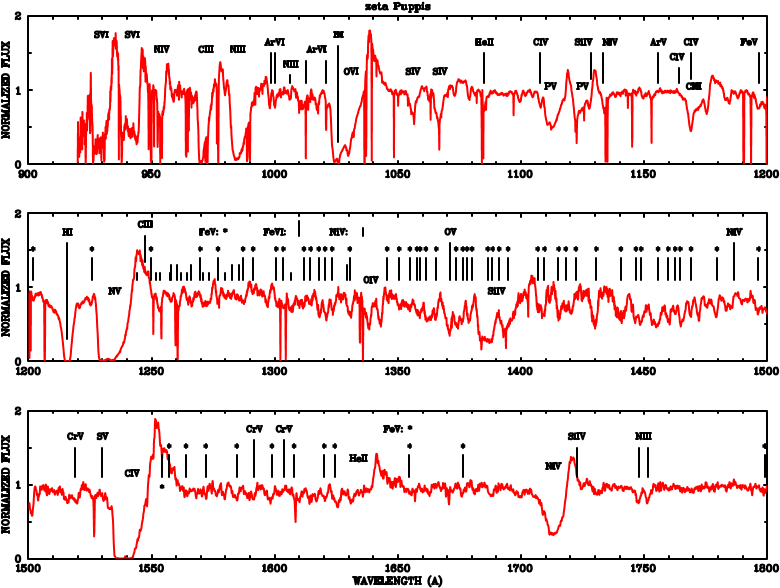
\includegraphics[width=1.0\textwidth]{figures/02-outflows/hot_star_wind.png}
\caption
[UV spectrum of one of the O4 supergiant $\zeta$ Puppis.]
{
{\sl Credit: Pauldrach et al. 1994}. 
UV spectrum of one of the brightest massive O stars, 
the O4 supergiant $\zeta$ Puppis. The spectrum is merged from 
Copernicus and IUE UV observations, and the prominent lines are 
marked.
} 
\label{fig:hot_star_wind}
\end{figure}

\subsubsection{Clumping in Stellar Winds}

\label{sec:clumpy_stellar}

Evidence for clumping in hot star winds comes from a range of sources.
Perhaps the most conclusive is from electron scattering wings
in emission lines; homogenous models overestimate the strength of these
wings, whereas clumpy models produce good agreement with data 
\citep{hillier1984,hillier1991eswingsmodel,hamann1992wr,hamann1994,schmutz1997}.
Further evidence for clumping comes from line variability \citep{prinja1992}
and polarisation \citep{brown1995}. Clumping is theoretically expected
in line-driven winds 
\citep[see section~\ref{sec:line_driving} and the review by][]{owocki2014}, 
and is directly dealt with in this thesis.
In chapter 5, I describe the treatment of clumping I have implemented 
in our radiative transfer code, before presenting
results from a clumpy AGN wind model.

\subsection{Outflow Physics}

The spectra in figures~\ref{fig:cordova}, \ref{fig:bals}
and \ref{fig:hot_star_wind} show striking similarities -- 
characteristic broad, P-Cygni-like absorption features in UV resonance
lines extending to high blueward velocities -- 
despite vast differences in mass, scale and the source of radiation. 
Furthermore, some of the phenomena observed in e.g. stellar winds may 
naturally solve some of 
the unanswered questions in other systems. For example, clumping
may prevent over-ionization in AGN outflows. It would seem
that at least some of the physics of outflows, like accretion physics,
is universal, and that lessons learned from smaller scale systems may be
scaleable to AGN and quasars. In order to understand if the similarity extends beyond
a cosmetic one, I will discuss some of the 
underlying physical mechanisms that may be responsible for accelerating
these outflows.

\section{Driving Mechanisms}

Let us consider a parcel of ideal gas. By imposing nothing more than
conservation of mass, energy and momentum on that parcel we can write down
three equations of magnetohydrodynamics (MHD):
% \footnote{I stress that these equations are not used in hydrodynamic
% simulations in this thesis (see chapter~5, for example); 
% they are discussed here because they provide a natural reference point
% for exploring potential driving mechanisms for winds in accreting systems.
% }

\begin{equation}
\label{eq:continuity}
\frac{D \rho}{Dt} + \rho \nabla \cdot \vec{v} = 0,
\end{equation}

\begin{equation}
\label{eq:motion}
\rho \frac{Dv}{Dt} = -\nabla P + \frac{1}{4 \pi}(\nabla \times \vec{B}) \times \vec{B} + \rho \vec{g}_{rad} + \rho \vec{g},
\end{equation}

\begin{equation}
\label{eq:energy}
\rho \frac{D}{Dt} \left(\frac{e}{\rho}\right) = P (\nabla \cdot \vec{v}) + \rho \cal{L}.
\end{equation}

Here $D$ denotes a derivative within the comoving frame of the gas parcel, $\vec{v}$ is the velocity,
$\rho$ is the gas density, $\vec{B}$ is the local magnetic field, $\vec{F}_{rad}$ is the radiation
force per unit mass, $\cal{L}$ is the cooling rate of the gas 
and $\vec{g}$ denotes the gravitational acceleration vector.

Equation~\ref{eq:continuity} is the {\em continuity equation} and describes conservation of mass. 
Equation~\ref{eq:motion} is the {\em equation of motion} and describes conservation of momentum.
Equation~\ref{eq:energy} is the {\em equation of energy conservation}. 
Equation~\ref{eq:motion} can be used to neatly demonstrate how an outflow can be driven. I have 
deliberately written the equation so that all the force terms lie on the RHS. 
For an outflow to be driven from an accreting object, one of the terms on the RHS must
dominate over gravity, $\rho \vec{g}$. These terms thus signify three potential
driving mechanisms.

\begin{itemize}
	\item Magnetic / Lorentz Forces, $\frac{1}{4 \pi}(\nabla \times \vec{B}) \times \vec{B}$.
	\item Radiative Forces, $\rho \vec{g}_{rad}$.
	\item Thermal Pressure, $-\nabla P$.
\end{itemize}

We can now examine under what physical conditions 
(and in which corresponding astrophysical objects)
we might expect these forces to overcome gravity and 
cause a parcel of mass to escape to infinity.
In other words: {\em what might drive a wind?}

\subsection{Thermal Winds}

In a disc in hydrostatic equilibrium (HSE), 
thermal pressure balances gravity in the vertical direction. 
The equation of motion in this $z$ direction can then be written as 
\begin{equation}
\label{eq:hse}
\rho \frac{Dv_z}{Dt} = -\frac{\partial P}{\partial z} +  \rho g_z = 0
\end{equation}
Clearly, if the thermal pressure is significantly 
increased, this equilibrium condition no longer holds. 
This can occur in accretion discs at temperatures in excess of $\sim10^7$~K --
where other forces are negligible compared to thermal pressure -- 
and where the escape velocities are relatively low (i.e. far out in the disc).
Due to the temperature and gravity scalings, this means
that XRBs are natural candidates for showing evidence of thermally driven
winds. The outer disc can be heated to the Compton temperature by 
the central X-ray source,
potentially driving relatively high mass-loss rate outflows 
\citep{begelman1983,woods1996}. 
This driving mechanism has been proposed as a natural explanation
for the ever-present equatorial outflows in soft state XRBs \citep{ponti2012}.
However, they are much less likely candidates in CVs and AGN, because
the escape velocity tends to greatly exceed the thermal velocity.

\subsection{Radiatively Driven Winds}
\label{sec:rad_winds}

Under spherical symmetry, one simply obtains the Eddington limit discussed
in section~\ref{sec:eddington} when $\rho \vec{F}_{rad} = \rho \vec{g}$. 
Hence, sources must be fairly close to the Eddington luminosity in order 
to drive an outflow purely from radiation 
pressure on electrons. There are a number of accreting systems that may drive
super-Eddington (or close to Eddington) outflows, 
such as AGN with UFOs \citep[e.g.][]{reeves2002,pounds2016},
NLSIs \citep{done2015} and ultra-luminous X-ray sources \citep[ULXs;][]{walton2013}.
However, high-state CVs are significantly below the Eddington limit 
\citep{warnerbook}, and at least some BALQSOs have low Eddington fractions 
\citep[$\sim25\%$ have $L/L_{Edd}<0.1$;][]{grupenousek2015}.
These systems may nevertheless be capable of radiatively driving strong 
strong radiatively driven outflows due to the influence of line opacity.
% Despite this, line opacity may mean that radiation is still responsible for the 
% powerful outflows in these systems even at $L / L_{Edd} \sim 10^{-3}$.

\subsection{Line-driven Winds}

\label{sec:line_driving}

Under the right ionization conditions, radiation pressure mediated by spectral lines
can be a significant  acceleration term in 
a partially ionized plasma \citep[][hereafter CAK]{CAK75}. 
The most common way to parameterise the cumulative
effect of lines on the radiation force is via the 
{\em CAK force multiplier}, ${\cal M}(t)$,
which modifies the equation for the acceleration due to radiation
to give \citep[][CAK]{castor1974}
\begin{equation}
\label{eq:force_multiplier}
\vec{g}_{rad} = \frac{\sigma_T F}{\mu c m_p} {\cal M}(t),
\end{equation}
where $F$ is the flux, and $\mu$ is the mean atomic weight.
${\cal M}(t)$ can be approximated by
\begin{equation}
\label{eq:force_multiplier2}
%% \cal{M}(t) = \sum_{lines} F_C \Delta \nu_D min (1/t, 1/\beta) 
{\cal M}(t) = t^{-\alpha} 
\left( \frac{n_e}{10^{11}~{\rm cm}^{-3}}\right)^\delta W^{-\delta},
\end{equation}
where $t$ is the dimensionless optical depth, given by
\begin{equation}
t = \frac{\sigma_T \rho v_{th}}{m_p | d(v_i) / ds |}
\end{equation}
% and $\beta$ is the ratio of the mass scattering coefficient of the free
% electrons, $\sigma_e$ to the line opacity, $\kappa_L$. $\Delta \nu_D$ is the Doppler
% width. 
Here $W$ is the dilution factor, and $k$, $\alpha$ and $\delta$ are constants with
values of 0.28, 0.56 and 0.99 respectively in O-star winds \citep{abbott1982}.
$v_i$ is the component of the velocity field in the direction
being considered, normally a line between the source of radiation and the wind.
It is possible to show \citep[CAK, ][]{owocki1988} that the maximum force multiplier
is around $2000-4000$. This is already an interesting result, as it tells us
that line-driven outflows can be accelerated when accretion rates / luminosities
are much lower than the Eddington limit. Indeed, using 
equation~\ref{eq:force_multiplier} we can see that a radiatively driven wind 
can be accelerated when $L_{UV} > L_{Edd} / M_{UV}(t)$, where the UV subscript 
pertains to the UV region of the spectrum and $M_{UV}(t)$ will thus depend on
the lines in this region and their relative ionization and excitation fractions.
Line-driven winds are present in O-stars and Wolf-Rayet stars and the theory
produces good matches with observations 
\citep[e.g.][]{friend1986,pauldrach1986,pauldrach1994,hamann2008}. 
It is also a strong candidate for driving
the winds seen in high-state CVs when the accretion disc is UV bright 
\citep[][see also section~\ref{sec:proga}]{pereyra1997,proga1998,proga2005}.

Line driving is also a promising mechanism to explain BAL outflows, as
the strong UV resonance lines seen in absorption in O stars are also 
present in BALQSOs. The presence of `line-locked' features \citep{bowler2014} 
and the `ghost of \la' \citep{arav1995, arav1996, north2006}
in the spectra of some BALQSOs also suggests that line-driving is
at least contributing to the acceleration of the wind 
\citep[but see also][]{cottis2010}.
However, the presence of an X-ray source complicates matters.
I have already briefly touched on the `over-ionization' problem
in AGN outflows, but it now has another consequence. Not only will 
strong X-rays prevent the right features forming in the spectrum, but, if
the outflow is line-driven, they will prevent the wind existing in the first 
place. Despite these problems, hydrodynamic simulations have been successful 
in producing high mass-loss rates (see section~\ref{sec:proga}).

Line-driving is subject to a strong instability known
as the line deshadowing instability 
\citep[LDI;][]{lucysolomon1970,macgregor1979,owockirybicki1984,owockirybicki1985}
The basic idea is that any velocity perturbation in a line-driven flow can cause a 
`deshadowing' effect, as the fluid element will now
be in resonance with a region of the spectrum that is less absorbed.
Thus, an increase in the line force will occur in proportion
with this velocity perturbation, and the instability can grow. 
Time-dependent numerical modelling of the LDI has shown that it can
produce a clumpy flow \citep{owocki1988,feldmeier1995,surlan2012,owocki2014}
that may explain the observational characteristics of clumping in 
stellar winds (see section~\ref{sec:clumpy_stellar}). 
The LDI is also of interest in CV and AGN winds, as it
may affect the ionization state of the flow and possibly the inferred
mass-loss rates.


\subsection{Magnetic Winds}
\label{sec:mag_winds}

There is still great uncertainty over the magnetic fields in accretion discs
and the physics of these magnetic processes. However, the MRI is one of the 
leading candidates for explaining angular momentum transport in accretion discs,
implying that magnetic processes are important in their dynamics. 
Thus, in many senses, magnetic driving is an attractive wind driving mechanism.
There are two main ways in which magnetic forces can drive an 
accretion disc wind, which are best explained by writing down an 
alternative form for the Lorentz force,
\begin{equation}
\vec{F_m} = \frac{1}{4\pi} \vec{B} \cdot \nabla \vec{B} - \nabla \frac{B^2}{8\pi}.
\end{equation}
The first term can be thought of as a magnetic {\em tension}
associated with the field lines and the second as an isotropic magnetic
{\em pressure}.

Historically, the most popular magnetic wind model has been 
the `bead on a wire' mechanism proposed by \cite{blandfordpayne} and 
\cite{pelletier_pudritz}. In these models, 
the poloidal magnetic field is dominant and is anchored in the 
accretion disc. A wind can then be driven by magnetic tension, as the
first term in the above equation operates on fluid elements (`beads') 
on the surface of the accretion disc. This can accelerate
a wind when the poloidal component of the field makes an angle of 
$>30^\circ$ with the normal to the disc surface. These models
are known as magnetocentrifugal winds as it is the interaction between
a centrifugal force and a strong, large-scale, ordered magnetic field 
threading the disc that drives the wind. 
Magnetocentrifugal winds have been proposed in both
AGN and YSOs \citep{pelletier_pudritz,konigl1994,kudoh1997},
and numerical simulations have demonstrated that this mechanism can produce
jets and outflows \citep{romanova1997,ouyed1997,ustygova1999}.

In an alternative magnetohydrodynamic (MHD) model the isotropic magnetic pressure 
is responsible for driving the outflow \citep{proga2003a}.
In this case the toroidal component dominates over the poloidal component
and drives a slow, dense outflow which behaves more like a thermally-driven wind 
(i.e. it conserves specific angular momentum rather than angular velocity). 

\section{Accretion Disc Wind Models}
\label{sec:wind_models}

A number of different wind models have appeared in the literature over the 
years, each attempting to explain the different observational characteristics
of quasars with a mixture of conceptual frameworks and underlying physics. 
Typically, the models attempt to explain the origins of BLR and BAL gas, although
some extend their remit into the infra-red, radio and X-ray regimes.
I will briefly discuss a few examples that have gained traction over the years,
before outlining the kinematic prescription I have used in the modelling that forms 
part of this thesis. 

\subsection{MCGV95: A Line-driven Wind Model for AGN}

\begin{figure}
\centering
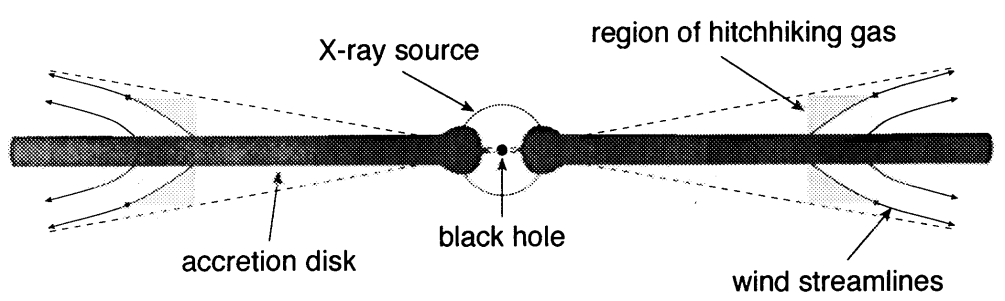
\includegraphics[width=1.0\textwidth]{figures/02-outflows/MCGV95.png}
\caption
[Cartoon showing the geometry of the MCGV95 model.]
{
{\sl Credit: Murray et al. 1995}. 
Cartoon showing the geometry of the MCGV95 model.
} 
\label{fig:MCGV95}
\end{figure}

MCGV95 proposed a model in which a smooth wind rises from an accretion disc with a launch
radius of around $10^{16}$~cm. The wind is equatorial, with an opening angle
of $5^\circ$, and is accelerated by line forces up to a terminal velocity of $0.1c$.
A sketch of the geometry is shown in Fig.~\ref{fig:MCGV95}.
One of the key features of the model is the presence of a `shield' of hitchhiking
gas, which protects the outflow from X-ray over-ionization 
and allows radiation pressure on UV resonance lines to efficiently 
accelerate the flow. 

MCGV95 found that BAL profiles were
seen for an observer looking into the wind cone, and significant collisionally excited
line {\em emission} emerged at low inclinations. This line emission came
from a relatively small BLR ($r_{BLR} \sim10^{16}$~cm) at the base of the wind, 
where densities were high ($n_e \approx 10^{10}$~cm$^{-3}$). 
The MCGV95 model was one of the first successful disc-wind unification models.
It is especially impressive as it includes photoionization calculations and 
quantitative estimates of the resultant line EWs. However, the effects of multiple
scattering and complex radiative transfer effects could not be included 
in the calculations (see chapter 5).

\subsection{De Kool \& Begelman: A Radiatively Driven, Magnetically Confined Wind}

It is, of course, possible that radiation and magnetic fields are both important
in determining the outflow characteristics. In the \cite{dekool1995} model, radiation
pressure drives an outflow from an accretion disc and also compresses the magnetic
field lines that are dragged along with the flow. This causes the magnetic field
strength in certain regions to be comparable to the gas pressure, meaning that clouds
can be magnetically confined in the flow. A diagram is shown in Fig.~\ref{fig:dekool}.
The authors find that such a model would naturally emerge at a fairly equatorial
angle with a covering factor of around $10\%$, and that lower ionization material 
would be intercepted when the system was viewed from higher inclinations, potentially
explaining some of the properties of LoBALQSOs.

\begin{figure}
\centering
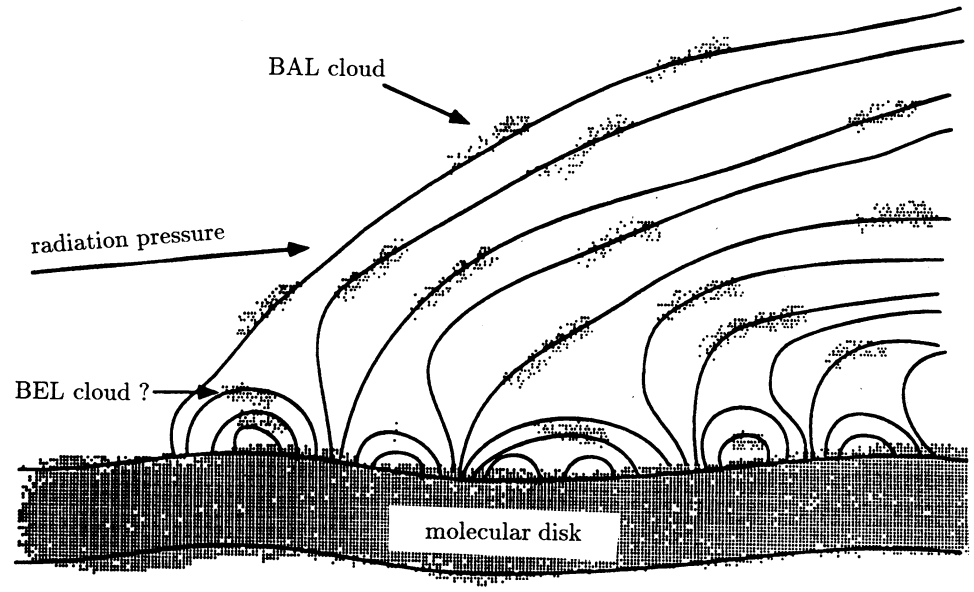
\includegraphics[width=1.0\textwidth]{figures/02-outflows/dekool.png}
\caption
[A cartoon showing the components in the De Kool \& Begelman model.]
{
{\sl Credit: De Kool \& Begelman 1995}. 
A cartoon showing the components in the De Kool \& Begelman model.
} 
\label{fig:dekool}
\end{figure}


\subsection{Elvis 2000: A Structure for Quasars}

\cite{elvis2000} expanded on the work of MCGV95 by proposing a simple
disc wind model, empirically derived to explain as much of quasar phenomenology
as possible within one unifying framework. The geometry of the Elvis'
is shown in Fig.~\ref{fig:elvis}. As in the two previous models, observers 
looking into the wind cone will see a BALQSO, whereas observers looking down onto
the wind will see a type 1 quasar. Initially, the wind rises vertically, so
that observers looking underneath the flow will see NALs
due to the small range of velocities intercepted by their line of sight. 

The flow conserves angular momentum, such that the initial Keplerian velocities
determine the BEL widths, before accelerating to BAL-like velocities of $\sim0.1c$.
The wind is assumed to be two-phase, with BEL and BAL clouds embedded in 
a warm, highly ionized medium (WHIM). This WHIM is responsible for WA-like absorption
and the X-ray scattering phenomena seen in AGN. It is also responsible for confining
the BAL and BEL clouds, allowing high densities and cooler temperatures to exist
within the flow. The ionization structure for the wind is stratified, such that the material
further out along the disc plane is somewhat shielded from the inner disc and X-rays.
This allows the lower ionization BEL profiles to form in the right locations,
and also means that LoBAL profiles would be seen at a subset of inclinations.

\begin{figure}
\centering
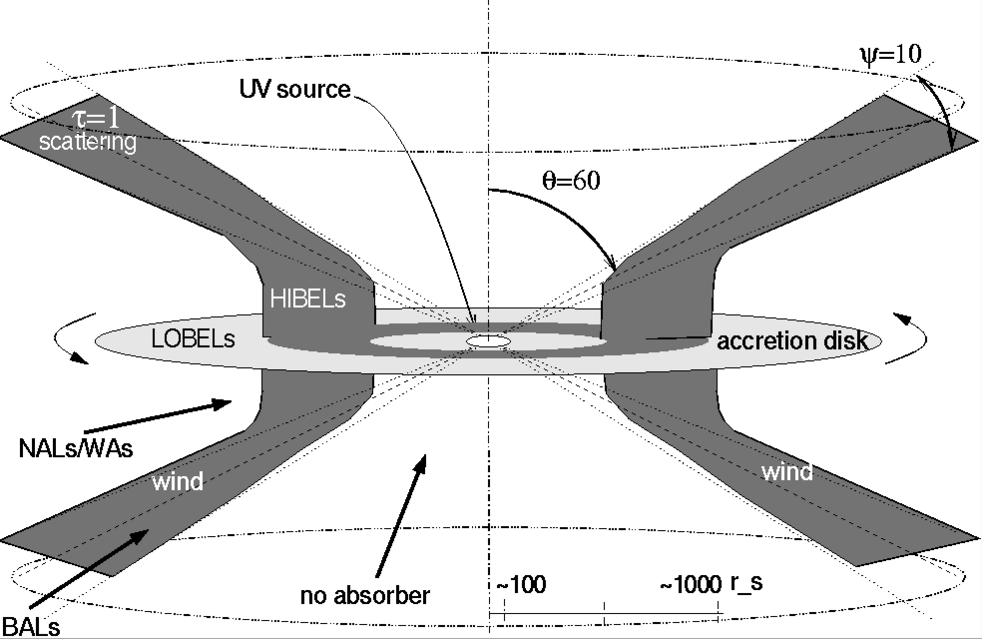
\includegraphics[width=1.0\textwidth]{figures/02-outflows/elvis.png}
\caption
[A schematic showing the main features of the Elvis model.]
{
{\sl Credit: Martin Elvis}. 
A schematic showing the main features of the Elvis model. A biconical
wind rises from an accretion disc, and the observed spectrum is determined 
purely by the viewing angle of the observer.
} 
\label{fig:elvis}
\end{figure}

\subsection{Proga et al.: Line-driven Hydrodynamic Models for AGN and CVs}
\label{sec:proga}

Around the turn of the century, Daniel Proga and collaborators 
published a series of important papers in which they conducted 
hydrodynamic simulations of live-driven disc winds in AGN and CVs. 
In the first of these, the problem considered was that of disc
winds in CVs \citep{proga1998}. In their model, the disc was assumed
to radiate according to the $\alpha$-disc model, and the central WD was also included
as a radiating source. They found that when the disc had an Eddington fraction 
of greater than $\approx 1 / {\cal M}_{max} (t) = 0.001$, then strong, line-driven
outflows were driven from a few WD radii with bending angles of $\sim45^\circ$.
This result agreed qualitatively with outflows in CVs, and later efforts to compute
synthetic line profiles produced promising results \citep{proga2002}. This was the
first successful demonstration of line driving in a full hydrodynamic simulation.

The same principle was then applied to the problem of AGN outflows, with the
additional complication of an ionization X-ray source now included 
\citep[][hereafter PK04]{PSK2000,PK04}. A density snapshot from the PK04 model
is shown in Fig.~\ref{fig:PK04}. An inner `failed' wind formed in this simulation,
which initially rose up from the disc before being over-ionized by the central X-rays.
Crucially, this acted as a shield, similarly to the hitchhiking gas proposed by
MCGV95, and allowed a line-driven wind to be accelerated further out in the disc. 
This outflow can be seen clearly in Fig.~\ref{fig:PK04}.

\begin{figure}
\centering
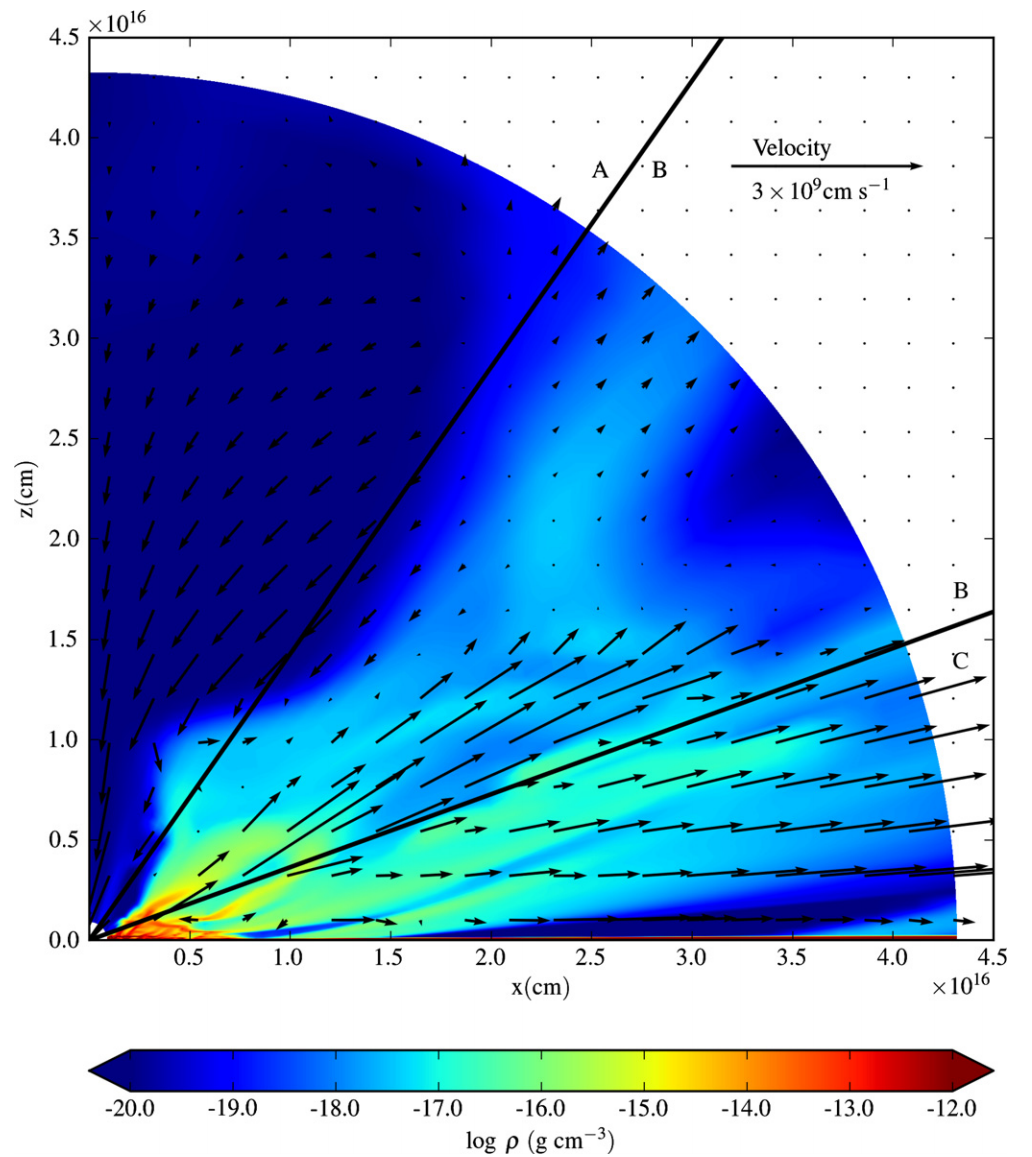
\includegraphics[width=0.8\textwidth]{figures/02-outflows/pk04_h14.png}
\caption
[Density snapshot of the PK04 model.]
{
{\sl Credit: Higginbottom et al. 2014.}. 
A snapshot of the PK04 model. Colours shows the density and 
arrows show the velocity of the flow. 
The radial lines separate three areas described by H14.
} 
\label{fig:PK04}
\end{figure}

One of the interesting results of the Proga-led simulations is that they tended
to produce somewhat unsteady, clumpy flows. In the CV case, this was caused by
the interaction between the line force and gravity, as both force terms varied 
differently with height. In the AGN case, it was instead due to the critical
importance of the ionization state on the line force. Parcels of gas can only 
be accelerated when if they have the `right' ionization state, and this depends
critically on their density and the radiation field they see. This causes
an interplay between the dynamics of the flow and the path of ionizing radiation, 
which are coupled. The radiation field also helped
determine the geometry of the outflow, as increasing the strength of the radiation
interior to the launch radius tends to flatten out the wind and lead to more
equatorial outflows \citep{proga2005}.
This is particularly important when considering quasar unification, as it means
the viewing angles of BALQSOs can provide information about where the wind is launched.

It is worth noting that the smaller scale LDI could not be included in this model,
partly for computational reasons and partly because of the approximations 
used to treat the radiation field. Treating the radiation transport is also
important for other reasons. 
\citet[][hereafter H14]{H14} showed that, in this particular geometry, 
multiple scattering renders shielding region
ineffective, and radiation will simply find its way around the failed wind
to over-ionize the flow beyond.
Ideally, full radiative transfer and hydrodynamical simulations would be used
to estimate the viability of line-driven winds. Our team is currently working 
on this problem (see H14 for the first step); however, much 
can also be learned from simpler, kinematic prescriptions for outflows, which
can then be treated with full radiative transfer and ionization treatments.  

\section{A Kinematic Prescription for a Biconical Wind}
\label{sec:sv93_model}

\citet[][hereafter SV93]{SV93} 
expanded on the work of the stellar wind community \citep[e.g.][]{AL85} 
in proposing a kinematic model for an accretion disc wind. Unlike 
hydrodynamical models, this model has no real predictive power in terms of velocities
and mass-loss rates. Instead, one sets these quantities in advance and examines the 
resultant properties of the flow and emergent spectra. The SV93 prescription
is the most common way of describing the outflow in the 
radiative transfer code \py\ (see chapter 3)
and has been used to simulate spectra for CVs \citep[][chapter 4]{LK02, M15}, 
AM CVn systems \citep{kusterer2014} and AGN/quasars 
\citep[][chapter 5]{higginbottom2013, M16, yong2016}. 
A similar philosophy applied to the model of \cite{KWD95}, which has been used
in similar applications \citep{LK02, simlong2008, sim2010}, as 
well as for young-stellar objects \citep[YSOs;][]{simmacro2005}.
Kinematic prescriptions have thus been a useful tool in providing quantitative
tests of conceptual models, and specifically for assessing their ability to reproduce
the observed spectra of a variety of disc wind systems.

In the SV93 parametrization,
a smooth, biconical disc wind emanates from the accretion disc between 
$r_{min}$ and $r_{max}$. A schematic is shown in Fig.~\ref{fig:sv93}.
The covering fraction of the outflow is 
also controlled by the inner and outer opening angles of the wind, $\theta_{min}$ and
$\theta_{max}$, and the launch angle of the other streamlines is given by 
\begin{equation}
\theta(r_0) = \theta_{min} + (\theta_{max} - \theta_{min}) \left(\frac{r_0 - r_{min}}{r_{max} - r_{min}} \right)^{\gamma},
\label{eq:wind_theta}
\end{equation}
where $r_0$ is the launch radius of the streamline.

\begin{figure}
\centering
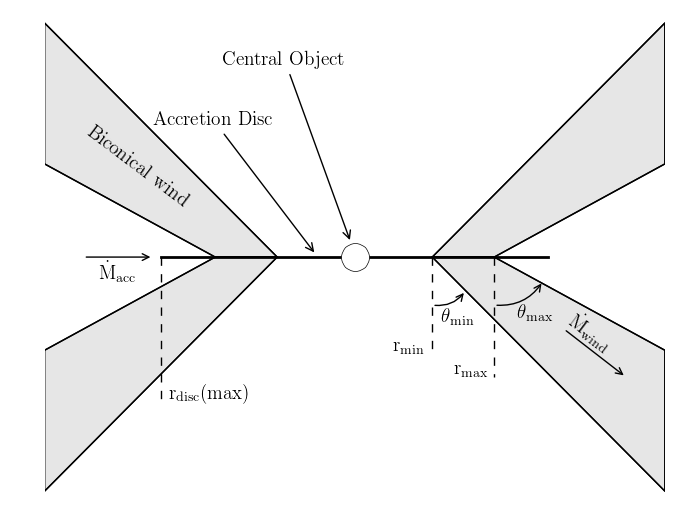
\includegraphics[width=1.0\textwidth]{figures/02-outflows/cartoon_general.png}
\caption
[A schematic showing the geometry and kinematics of the SV93 model]
{
A schematic showing the geometry and kinematics of the SV93 model. 
} 
\label{fig:sv93}
\end{figure}

The poloidal (non-rotational) velocity field of the wind, $v_l$, is given by
\begin{equation}
v_l=v_0+\left[v_{\infty}(r_0)-v_0\right]\frac{\left(l/R_v\right)^{\alpha}}{\left(l/R_v\right)^{\alpha}+1},
\label{eq:v_law}
\end{equation}
where $l$ is the poloidal distance along a particular wind
streamline. The terminal velocity along a streamline, $v_{\infty}$, is
set to a fixed multiple of $v_{esc}$, the escape velocity at the launch
point. The terminal velocity will therefore be higher for streamlines closer
to the inner disc edge.
The launch velocity from the disc surface, $v_0$, is assumed to
be constant (set to $6$~km~s$^{-1}$). Once the wind is launched, it
accelerates, reaching half of its terminal velocity at $l = R_v$. The
velocity law exponent $\alpha$ controls how quickly the wind
accelerates. Larger values of $\alpha$ cause the main region of 
acceleration to occur close to $R_v$, whereas smaller values
correspond to fast acceleration close to the disc (see
Fig.~\ref{acc_law}). The rotational velocity $v_\phi$ is 
Keplerian at the base of the streamline 
and the wind conserves specific angular momentum, such that
\begin{equation}
v_\phi r = v_{k} r_0,
\label{eq:vrot}
\end{equation}
where $v_{k}=(GM_{WD}/r_0)^{1/2}$.

The mass-loss rate per unit surface area, $\dot{m}^\prime$,
can be controlled by a free parameter $\lambda_m$ such that
\begin{equation}
\dot{m}^\prime \propto \dot{M}_W~r_0^{\lambda_m} \cos [\theta(r_0)],
\label{eq:dmda}
\end{equation}
where $\dot{M}_W$ is the total mass loss rate in the wind. This equation is normalised so 
that when integrated over both sides of the disc the correct $\dot{M}_W$ emerges.
I have adopted $\lambda=0$ throughout this thesis, which corresponds to uniform
mass loss across the disc.
The density at a given point can then be calculated by imposing mass conservation
and using the velocity law. At the base of the wind, the density is 
given by
\begin{equation}
\rho (r_0) = \frac{\dot{m}^\prime(r_0)}{v_z(r_0}.
\label{eq:rho0}
\end{equation}
At a coordinate $(r,z)$ in the wind, the density is then
\begin{equation}
\rho (r, z) = \frac{r_0}{r} \frac{d r_0}{dr}\frac{\dot{m}^\prime(r_0)}{v_z(r,z)}
\label{eq:rho_rz}
\end{equation}
where the corresponding $r_0$ is found by considering the streamline that 
passes through $(r,z)$. These equations govern the kinematics
and densities in the wind in the SV93 prescription, which is used
extensively throughout this thesis. 
% This prescription is used to describe the outflow in
% the radiative transfer code \py. 
% The radiative transfer procedure and 
% ionization calculation is described in chapter 3, and specific
% applications of this model are described in
% chapters 4 and 5.


\begin{figure}
\centering
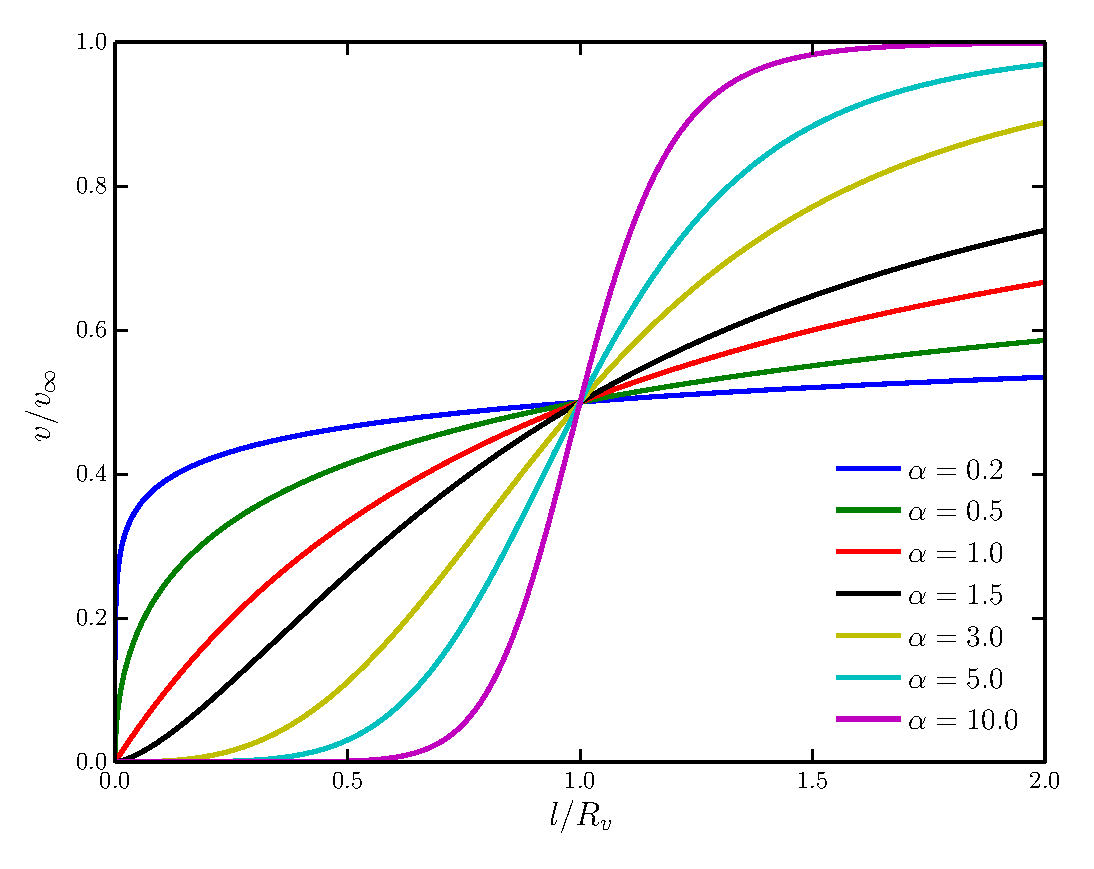
\includegraphics[width=1.0\textwidth]{figures/05-cvpaper/acc_law.eps}
\caption
[The SV93 velocity law for various values of the
acceleration exponent, $\alpha$.]
{
The SV93 velocity law for various values of the
acceleration exponent, $\alpha$.
%%{\bf JM: KSL has suggested we ditch this}
} 
\label{acc_law}
\end{figure}




\section{The big picture: AGN Feedback}
\label{sec:agn_feedback}

The event horizon of a $10^9~M_\odot$ BH is approximately 
$10^{15}$~cm, a billionth of the radius of a typical galactic bulge. This is 
roughly the ratio in size between a small coin and the 
Earth. Even the sphere of gravitational influence of the BH is roughly 
$1000$ times smaller than the size of the galactic bulge.
Despite this vast different in scale, there is strong evidence
that the physics on the scale of the gravitational
radius of the BH affects the evolution and dynamics of its host galaxy.
This becomes less surprising when considering the {\em energetics} of accretion.
The binding energy of a galactic bulge, with mass 
$M_{bulge}$ and velocity dispersion $\sigma_*$, is 
\begin{equation}
E_{bulge} \approx M_{bulge} \sigma_*^2,
\end{equation} 
while the energy released in growing a black hole to a 
mass $M_{BH}^\prime$ is (equation~\ref{eq:restmass}, assuming $\eta=0.1$)
\begin{equation}
E_{BH} \approx 0.1 M_{BH}^\prime c^2.  
\end{equation}
By combining these two equations, and substituting in typical numbers 
($\sigma_* = 0.001c$, $M_{BH}^\prime / M_{bulge} = 10^{-3}$), we can show that 
\begin{equation}
\frac{E_{BH}}{E_{bulge}} \approx 10^{-4} \left( \frac{c}{\sigma_*} \right)^2 \sim 10.
\end{equation}
In other words, the energy released when growing a BH can significantly exceed
the binding energy of the galactic bulge. This energetic 
argument is, of course, not sufficient to claim that the accreting BH must affect its
host. For example, if the radiated energy never experienced an 
optical depth of $\sim 1$, it could not couple to the galactic bulge. However,
we have already seen that many outflows in AGN possess kinetic luminosities that
are significant compared to the bolometric luminosity. Thus, outflows 
(and jets) may provide a mechanism by which the vast accretion energies can
be transferred to the BH environment.

\subsection{Observational evidence for feedback}

Perhaps the most famous pieces of evidence for some kind of long-distance 
relationship between a central BH and its host galaxy are the 
$M_{BH}-\sigma_*$ \citep{ferrarese2000,gebhardt2000,gultekin2009} and $M_{BH}-M_{bulge}$ 
\citep{magorrian1998,haring2004,mcconnell2013} correlations, 
shown in Fig.~\ref{fig:msigma} and Fig.~\ref{fig:mbulge}, respectively.
By themselves, these correlations would not necessarily imply
that the AGN is having an impact on its environment. Indeed, there are many different
theoretical models for the origin of these relations 
\citep[e.g][]{somerville2001,adams2001,burkert2001,king2003,croton2006,kormendy2013}. 
However, there are many other clues that outflows and jets from AGN can affect
the host galaxy evolution and morphology.

\begin{figure}
\centering
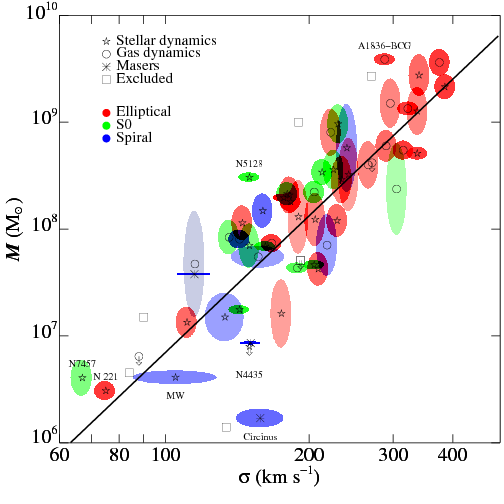
\includegraphics[width=0.7\textwidth]{figures/02-outflows/msigma.png}
\caption
[The $M_{BH}-\sigma_*$ correlation.]
{
{\sl Credit: Gultekin et al. 2009}. 
The $M_{BH}-\sigma_*$ correlation.
} 
\label{fig:msigma}
\end{figure}

\begin{figure}
\centering
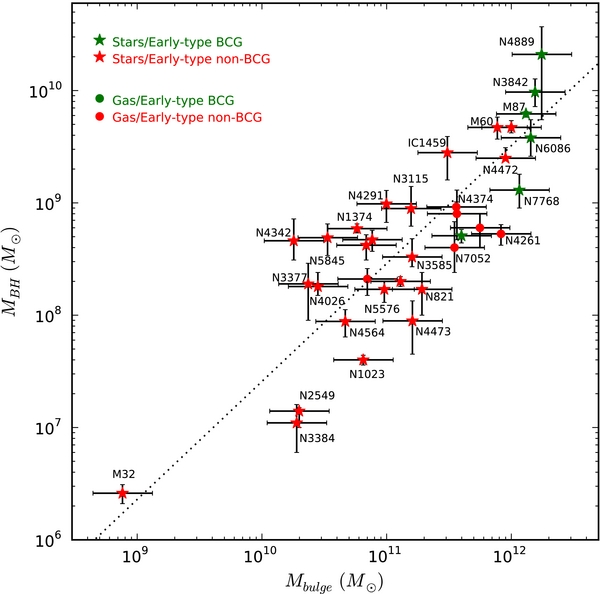
\includegraphics[width=0.7\textwidth]{figures/02-outflows/mbulge.jpg}
\caption
[The $M_{BH}-M_{bulge}$ correlation.]
{
{\sl Credit: McConell \& Ma 2013}. 
The $M_{BH}-M_{bulge}$ correlation.
} 
\label{fig:mbulge}
\end{figure}

The galaxy luminosity function describes
the number of galaxies as a function of luminosity and is generally modelled
with the \cite{schechter1976} function. Theories of 
galaxy evolution tend to overpredict the number of galaxies at the
high luminosity end, which can be avoided by invoking quenching
of star formation by the central AGN \citep[e.g.][]{read2005,bongiorno2016}.
Galaxies also show bimodality in their colour distributions 
\citep{strateva2001,bell2003a,baldry2004}, 
with a clear separation between a blue, star-forming
main sequence, and a red sequence with lower 
specific star formation rate (sSFR). Furthermore, these two 
sequences tend to lie in the same regions of colour space as the 
host galaxies of high and low 
Eddington fraction AGN respectively, implying that the AGN may be 
directly responsible for quenching the star formation and moving 
a galaxy onto the `red and dead' branch. This has been demonstrated in 
several numerical simulations \citep[e.g.][]{springel2005,croton2006}.

There is also evidence that AGN are energetically 
significant on scales larger than the galactic bulge. X-ray observations
of cool core clusters and elliptical galaxies
can show dramatic X-ray cavities or bubbles
up to 50~kpc across, with a radio-loud AGN at the centre
\citep[Fig.~\ref{fig:xray_bubbles}]{randall2011,cavagnolo2011,fabian2012}. This
shows how radio jets can significantly impact the surrounding gas,
a flavour of feedback known as `radio' or `kinetic' mode.
These cavities also provide an estimate of the kinetic power of a radio
jet, as the volume of the bubble and surrounding gas pressure gives a 
rough estimate of the $PV$ work done by the jet. This can be divided by
an age estimate for the cavity, giving powers
of up to $10^{46}$erg~s$^{-1}$, which are weakly 
correlated with the radio luminosity of the source, 
and can be large for modest radio power \citep{birzan2008}. 

\begin{figure}
\centering
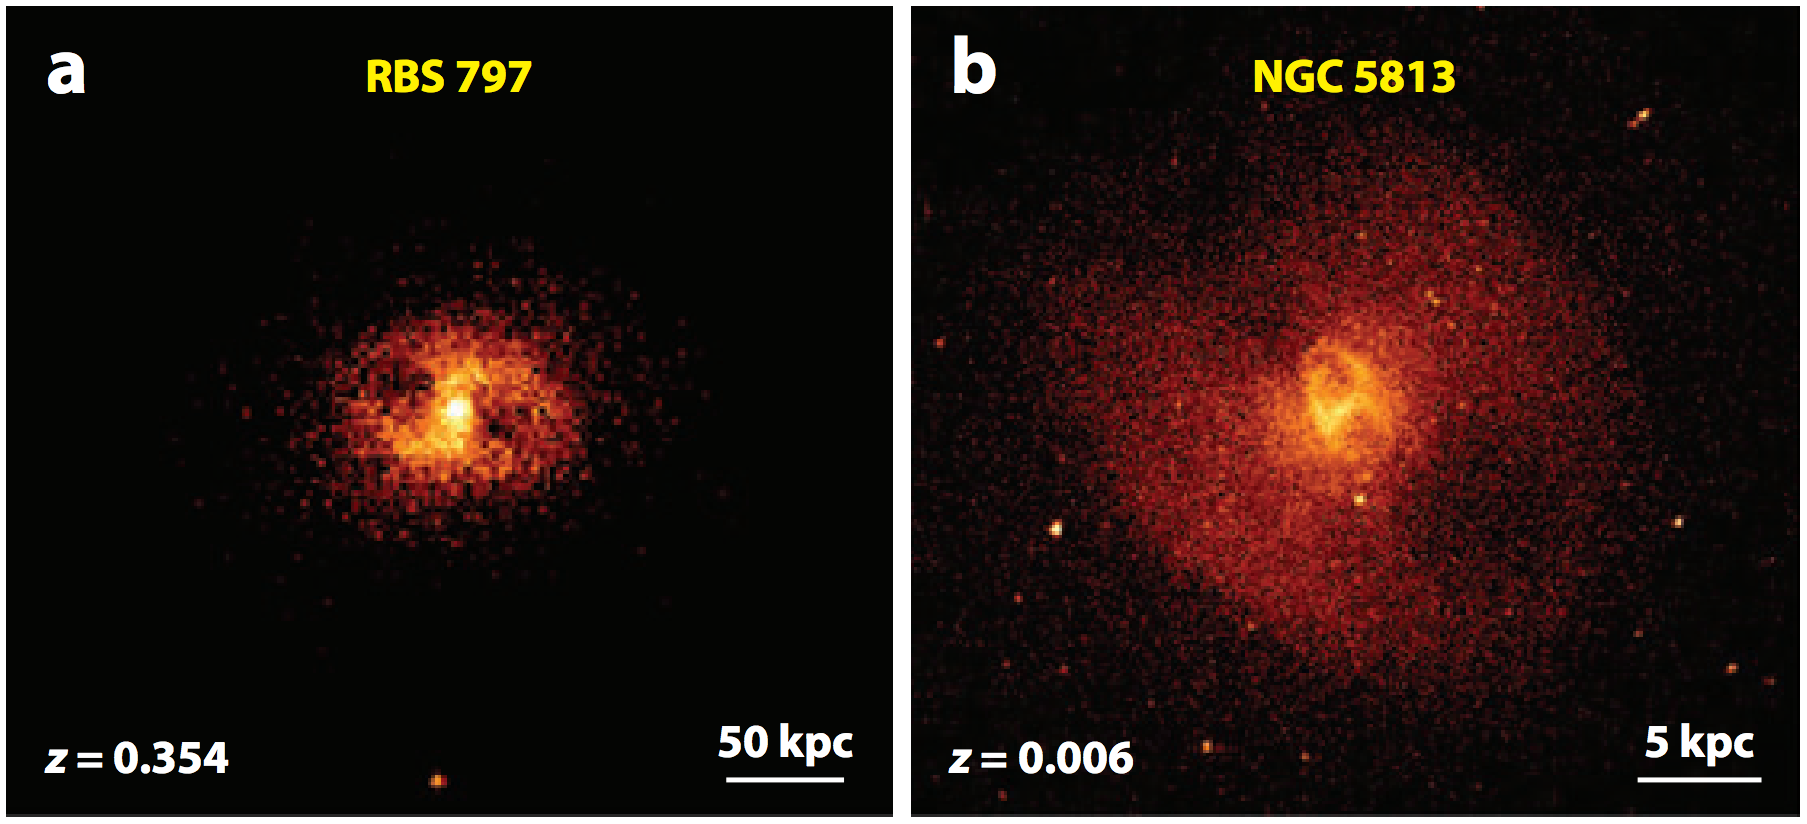
\includegraphics[width=1.0\textwidth]{figures/02-outflows/xray_cavities.png}
\caption
{
{\sl Figure adapted from Fabian 2012}. 
{\sl Chandra} X-ray images showing two examples of X-ray cavities,
illustrating how a radio jet from an AGN can have a dramatic impact 
on its environment. a) The RBS 797 Cluster (Cavagnolo et al. 2011). 
b) elliptical galaxy NGC 5813 (Randall et al. 2011).
} 
\label{fig:xray_bubbles}
\end{figure}

However, jets are not the only way for AGN to interact with 
their environment. I have already briefly discussed in section~\ref{sec:ufos}
how fast AGN winds can drive larger-scale molecular outflows.
This can be seen spectacularly in the FeLoBALQSO Mrk231, 
where integrated field spectroscopy shows kiloparsec-scale
neutral gas outflows \citep[see Fig.~\ref{fig:rupke};][]{rupke2011}.
Furthermore, \cite{king2003} expanded on the ideas of \cite{silkrees1998} and
considered a super-Eddington, momentum-driven outflow expanding into the surrounding gas. 
This model naturally reproduces the observed slope of the $M_{BH}-\sigma_*$
relation. This line of argument was used to suggest that super-Eddington accretion must be
common near the end of a quasar cycle, although it is worth noting that line-driving,
or non-radiative driving, would mean that super-Eddington accretion rates are 
not required to drive such an outflow. Intriguingly, this means that 
understanding outflow physics has implications for the \cite{soltan1982} argument,
SMBH spin and the accretion history of the Universe.

\begin{figure}
\centering
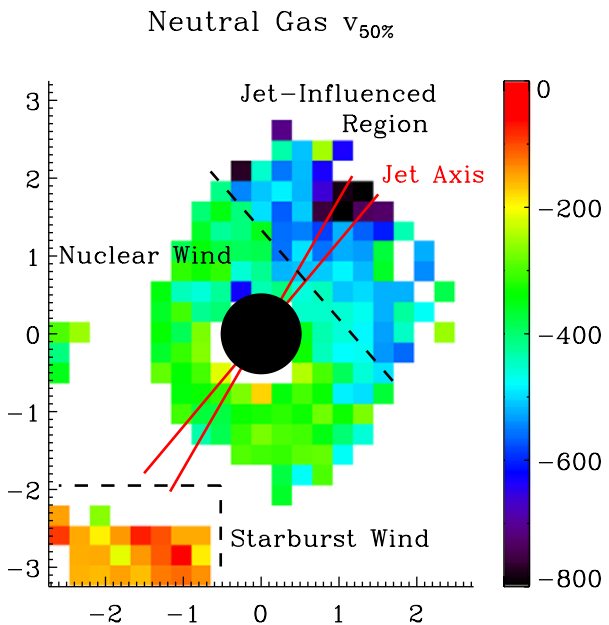
\includegraphics[width=0.8\textwidth]{figures/02-outflows/rupke2.png}
\caption
[Results of Gaussian line profile fitting to 
integral field spectroscopy of Mrk 231.]
{
{\sl Credit: Rupke \& Veilleux 2011}. 
Results of Gaussian line profile fitting to 
integral field spectroscopy of Mrk 231. The quantity
shown, $v_{50\%}$, corresponds to the centre of the fitted Gaussian
profile and indicates that high outflow velocities 
are present in the neutral gas.
} 
\label{fig:rupke}
\end{figure}


\subsection{Alternative Explanations}

It cannot yet be proven that AGN are the drivers of the observed 
galaxy colour evolution, high-end luminosity function discrepancy or
BH-bulge correlations. 
In particular, it is also possible that mergers are responsible for these phenomena. 
For example, major galaxy mergers may explain the `red and dead' branch
of the galaxy colour bimodality \citep[e.g.][]{somerville2001,baldry2004}. 
However, AGN winds and jets are clearly 
energetically significant with respect to their host galaxies, so estimating
their kinetic powers accurately is important in discriminating between in-situ
and ex-situ scenarios. 

Having established the astrophysical importance of outflows, 
I will now move on to discussing how we might go about 
accurately modelling the ionization states of accretion disc winds, 
and their emergent spectra.


